\section{Load Dependence}
\label{sec:load}

A negative result about adaptivity invites the obvious objection: adaptivity
pays when conditions \emph{change}, and a single stationary trace is the one
case where a static cap should be near-optimal. We agree, and we test it.

We run the same controller and the same cap family on a 25-session tier. The
throttle configuration is reversed: with all safety throttles disabled, the
25-session tier runs \emph{51\% faster} (58.4 to 28.8 minutes) at a cost of
only 2.4\,pp of SLO, while on the 200-session tier disabling the same
throttles costs 42\% (291.3 to 415.0 minutes) and 43.7\,pp of SLO. One switch,
two regimes, opposite signs, both around 40--50\%
(Fig.~\ref{fig:loadtier}). No single scalar setting is optimal across both.

This is the regime in which adaptive control should win, and we report two
findings about it. The first is discouraging for our controller: on the
25-session tier it does not win. A static cap of three, re-run under the
current harness, finishes in 24.2 minutes at 91.2\% SLO---16\% faster than the
most aggressive \sys{} configuration we measured on that tier, and with better
run-to-run stability (segment SD 5.1 against 11.0 for cap-2). The stateless
cap, which cannot see occupancy, backlog or remaining work, is simply better
here. We flag one caveat and one gap. The caveat is that the tier comparison
above is cross-generation: the 25-session throttle arms come from an earlier
harness revision and are not directly comparable to the 200-session numbers,
so we treat them as a direction rather than a magnitude. The gap is that the
matching \sys{} arm on the 25-session tier under the current harness was
interrupted by another tenant and is not reported.

The second finding is the more useful one. The signal an adaptive controller
would need is available---the number of sessions waiting for admission differs
by 6--7$\times$ between the tiers (median 9--11 at 25 sessions against 66 at
200, maximum 135)---but its \emph{interpretation} is not obvious. At the
25-session tier the controller holds eleven sessions back while running
exactly one; that backlog is manufactured by the throttling itself rather than
evidence that demand has slackened. Reading it correctly requires combining
instantaneous backlog with progress through the run, which is a stateful
computation a cap cannot perform. We regard this as the most promising
direction we did not finish, and we are explicit that we did not finish it.

\begin{figure}[tb]
  \centering
  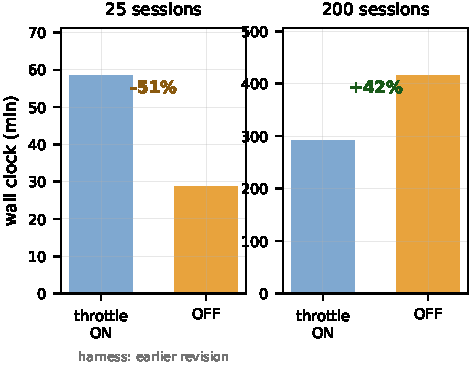
\includegraphics[width=\columnwidth]{figs/fig5_loadtier.pdf}
  \caption{The same throttle switch, two load tiers, opposite signs. The
  25-session bars are from an earlier harness revision and are shown as a
  direction, not a magnitude; the matching current-harness arm was interrupted
  and is not reported.}
  \label{fig:loadtier}
\end{figure}

\section{Related Work}
\label{sec:related}

\paragraph{Admission and scheduling for agentic serving.} Recent systems
report large gains from treating an agent session, rather than a request, as
the schedulable unit, and from preserving session state across tool calls:
session-aware admission with CPU-restorable KV
\cite{talaria,continuum}, program-level pause/resume with shortest-context-first
restoration \cite{thunderagent}, and congestion-based control over an
agent-level window \cite{concur}. A recurring measurement in this line is that
recomputation, not admission, dominates: \cite{concur} attributes 49.1\% of
end-to-end latency to recomputation, and \cite{mori} preserves state on the
CPU at the cost of a reload. Our results are consistent with this literature
rather than in tension with it, and \S\ref{sec:discussion} explains why: the
mechanism these systems add is one our controller already has.

\paragraph{Engine-side techniques.} A separate line improves the engine
rather than the admission decision. Iteration-level batching and paged KV
\cite{yu2022orca,kwon2023pagedattention} are the substrate every policy here runs
on; chunked prefill with stall-free batching \cite{sarathi}, prefill/decode
disaggregation \cite{distserve}, and cache-centric scheduling
\cite{mooncake} are the refinements. Our \S\ref{sec:model} attributes 7--10\,ms of each
26\,ms step to non-decode work, which is exactly what this line attacks. We
emphasise that these techniques raise the achievable rate for \emph{all}
policies; they move the frontier rather than deciding who sits above it.

\paragraph{State retention and preemption.} A third line keeps session state
alive across the gaps we measure in \S\ref{sec:model}: keeping KV on cheaper
storage across turns \cite{yu2025pensieve,gao2024cachedattention}, migrating it
between instances \cite{sun2024llumnix}, and preempting at iteration granularity
\cite{wu2026fastserve}. These systems exercise finer control than our 2\,s
admission cycle, which is the boundary of our negative result: we falsify one
control granularity, not the family. What they share with \sys{} is that the
state is not discarded---which is why, as we argue below, adding admission
intelligence on top buys nothing here.

\paragraph{Application-level dependencies and replay.} Serving an LLM
\emph{application} rather than a request means the scheduler sees dependencies
between calls \cite{lin2024parrot}, and agentic traces have structure that
request-level benchmarks do not capture \cite{wang2026xperf}. Our replay
preserves that structure but fixes it in advance, which is exactly the
limitation these works would press on.

\paragraph{Prefix caching.} The prefix cache is often proposed as the signal
an admission policy should use. In our workload it is not a policy variable:
round-1+ hit rate equals the trace's own planned value (89.8\%) to within one
percentage point across four different admission policies, so admission does
not move it. We note the boundary of this claim---we varied admission policy,
not eviction policy, and SGLang exposes alternate eviction policies we did not
test, and production KV-cache traces show hit rate is sensitive to policy in
ways a single trace family may not reveal \cite{wang2025kvcachewild}.

\section{Discussion}
\label{sec:discussion}

\paragraph{Why published gains do not reappear.} The systems cited above win
by preserving session state across tool waits and by pausing at agent
granularity. \sys{} inherits both properties from its permit design: a session
holds its permit for its whole lifetime and its KV is preserved across waits,
and the permit file supports the same pause primitive \cite{concur} uses. If
that mechanism is where the published gains come from---and the measurements
in those papers suggest it is---then a controller that already has it has
nothing left to add by admitting more cleverly. This reframes our negative
result: it is not that admission control cannot work, but that on this workload
the mechanism that makes it work has already been spent.

\paragraph{A criterion, not just a verdict.} The decomposition suggests a
cheap test for whether admission control can pay on a given workload. Measure
$\overline{R}$ and $\tau$ (by Method 2, which needs only per-request logs) over
a range of concurrency. If $\tau$ is flat, raising $\overline{R}$ converts
directly into wall clock and admission control has room. If $\tau$ rises
proportionally with $\overline{R}$, the two cancel and it does not. Our 13
measured configurations give 18.4--32.2\,ms across a running range of
0.64--1.62, i.e.\ a rise of 13.8\,ms over 0.98---a factor of 1.75 against a
concurrency factor of 2.5, which absorbs more than half the gain.
We offer this as the paper's constructive output, and we note it is testable
in minutes on a system that already logs per-request timings.

\paragraph{Limitations.} Our results come from one 24\,GB accelerator, one 7B
model and one trace family; generality is untested. Two specific boundaries
matter. First, the pool holds about four median sessions, so concurrency is
capacity-bound by construction; on a device with a much larger pool the
premise may not hold and the conclusion may invert---we regard reproducing on
a larger device as the single most important next experiment. Second, the
load is stationary, single-tenant and single-SLO. The load-dependence result
of \S\ref{sec:load} says the reverse should be expected when conditions vary,
and multi-tenant or heterogeneous-SLO settings are where we would look next.

\paragraph{Reproducibility.} Every verdict in this paper is produced by one
script from the raw per-step logs, and every run is guarded against a shrunken
KV pool. We report three claims we retracted during the work, because the
retractions were the most informative events: a median-based reading of the
tool wait that inverted a central assumption, a growth-sensitivity conclusion
that rested on an arm we had already invalidated, and the accounting
double-charge of \S\ref{sec:results}, falsified twice---once by source
inspection and once by the end-to-end measurement here.

\section{Conclusion}

We asked whether an adaptive admission controller can beat a tuned static
concurrency cap on a memory-bound agentic LLM workload, and found that on our
system it cannot: nine variants, four mechanistically distinct routes, none
above the static front. The reason is a cancellation. Admission policy controls
how many requests are in flight; the per-step cost rises with that number; and
the product is what the wall clock sees. We gave a two-part decomposition of
the wall clock that makes the cancellation measurable, identified a structural
idle component the policy cannot recover, and showed the regime in which
adaptivity should have paid---where the same switch is worth $+51\%$ and
$-42\%$---is one where a stateless cap still wins. The constructive output is a
per-request measurement that decides, in minutes, whether admission control
has room on a given workload.
